%!TEX root = ../template.tex
%%%%%%%%%%%%%%%%%%%%%%%%%%%%%%%%%%%%%%%%%%%%%%%%%%%%%%%%%%%%%%%%%%%%
%% my-chapter1.tex
%% NOVA thesis document file
%%
%% Chapter with the template manual
%%%%%%%%%%%%%%%%%%%%%%%%%%%%%%%%%%%%%%%%%%%%%%%%%%%%%%%%%%%%%%%%%%%%
%\usepackage{amsmath}
%\usepackage[table]{xcolor}
%\usepackage{xltabular}
%%\usepackage{colortbl} % Added this line
%\usepackage{booktabs}
%\usepackage{enumitem}
%\usepackage{tikz}
%\usetikzlibrary{shapes, arrows, positioning, fit}


\typeout{NT FILE mfc.tex}%

\chapter{Computational Financial Mathematics}
\label{ch:comp_fin_math}

    This assignment for the Computational Financial Mathematics course explores and applies various financial
    modelling and computational techniques.
    The project encompasses key topics such as financial mathematics, discrete-time and continuous-time modelling,
    partial differential equations, Monte Carlo simulation, and sensitivity analysis.
    The Binomial model for option pricing will be examined, and the Black-Scholes model will be derived and implemented.
    Option pricing problems will be solved using PDEs,
    and Monte Carlo simulations will be used to model asset price evolution.
    The Greeks for European options will be computed.
    Practical examples and computational implementations will be demonstrated using Python,
    ensuring a comprehensive understanding of the concepts covered.

\section{Financial Mathematics}
    \label{sec:fin_math}

%    Review and describe the main concepts of financial mathematics,
%    namely the concepts of Equities, Commodities, Forwards, Futures and Options.

    Financial mathematics is a branch of applied mathematics that deals with financial markets and instruments.
    It is a fundamental tool for understanding and analysing financial markets, pricing financial instruments,
    and managing financial risk.
    Key examples include equities, commodities, forwards, futures, and options.
    These concepts are essential for understanding the functioning of financial markets and the valuation of
    financial instruments.
    They are built upon core concepts such as the time value of money, risk and return, and arbitrage.
    Financial mathematics provides the tools and models to analyse these assets and understand their behaviour in the market.

    \subsection{Equities}
        \label{sec:equities}

        Equities, also known as stocks or shares, represent ownership in a company.
        When an investor buys shares of a company,
        they become a part-owner of the company and are entitled to a share of the company's profits.
        Equities are traded on stock exchanges, and their prices are determined by supply and demand in the market.
        Traditional Equity investors can make money through:

        \begin{itemize}
            \item Capital appreciation: Investors buy shares with the expectation that the value will increase over time,
                allowing them to sell at a higher price and realise a profit.
            \item Dividends: Companies distribute a portion of their profits to shareholders in the form of dividends.
            \item Short selling: Investors can also make money by selling borrowed shares with the intention of buying
                them back at a lower price.
            \label{item:equity_investing}
        \end{itemize}

        In addition to traditional equity investments,
        investors can also invest in equity derivatives, such as options and futures,
        which allow them to speculate on the price movements of equities without owning the underlying shares.

    \subsection{Forwards}
        \label{sec:forwards}

        A forward contract is a financial agreement between two parties to buy or sell an asset at a predetermined price,
        with the transaction set to occur at a specified future date.
        The contract price is established at the time the agreement is initiated.
        Forward contracts play a significant role in managing financial risk,
        particularly as a hedge against adverse price fluctuations,
        while also serving as a vehicle for speculation on future pricing trends.
        One of the key advantages of forward contracts lies in their flexibility,
        as they can be tailored to the unique requirements and preferences of the parties involved.

    \subsection{Futures}
        \label{sec:futures}

        A futures contract shares similarities with a forward contract in its purpose and structure;
        however, it differs by being standardised and traded on a regulated exchange.
        These standardised terms ensure greater transparency and facilitate market efficiency.
        Futures contracts are widely used in financial markets for two primary purposes: hedging,
        where they help mitigate the risks associated with price fluctuations, and speculation,
        where they allow participants to express views on future price movements\cite{hull_options_2012}. \\

        One of the primary advantages of futures contracts is their high liquidity,
        stemming from the fact that they can be easily bought or sold on an exchange.
        This liquidity enhances their appeal to market participants,
        particularly those seeking flexibility in managing risk or capitalising on market opportunities.
        Moreover, these instruments are used across a broad spectrum of markets, encompassing commodities, equities,
        and interest rate derivatives, highlighting their versatility and significance in modern financial markets. \\

        Table~\ref{tab:futures_forwards} outlines the key differences between futures and forwards contracts:

        \begin{xltabular}{\textwidth}
            {   % This is the column specification for the table
                >{\ttfamily\raggedleft\arraybackslash}m{0.33\textwidth}
                >{\ttfamily\centering\arraybackslash}m{0.33\textwidth}
                >{\ttfamily\centering\arraybackslash}m{0.33\textwidth}
            }
            \hline
                                & \textbf{Futures} & \textbf{Forwards} \\
                \hline
            \textbf{Contract}    & Highly standardized & Custom \\
                \hline
            \textbf{Exchange}    & Established & OTC \\
                \hline
            \textbf{Mark to Mkt} & Yes & No \\
                \hline
            \textbf{Settled @}   & Ending price ($P_T$) & Contract price ($F_0$) \\
                \hline
            \textbf{Credit risk} & No (counter party is clearinghouse) & Yes \\
                \hline
            \textbf{Duration}    & Traded continuously & Held until maturity \\
                \hline
            \textbf{Cash flow}   & Daily + Margin Req. & At delivery \\
            \hline
            \label{tab:futures_forwards}
        \end{xltabular}

    \subsection{Commodities}
        \label{sec:commodities}

        Commodities represent fundamental raw materials or primary agricultural products
        that serve as the foundation of global trade and economic activity.
        Examples include metals such as gold, energy resources like oil,
        and agricultural products such as wheat and coffee. These assets are traded on organised commodity exchanges,
        where their prices are governed by the dynamic interplay of supply and demand.
        The inherent volatility in commodity prices is influenced by a variety of factors,
        including weather variability, geopolitical uncertainties,
        and shifts in global economic conditions\cite{wilmott_paul_2007}.
        Understanding and modelling such price behaviour,
        particularly through quantitative methods rooted in mathematics and statistics,
        is of critical importance in developing robust risk management and trading strategies

%    In practice, turbine manufactors provide a table of values for the power output at discrete wind speeds.
%    Within the range of these two critical thresholds,
%    the relationship between wind speed and the generated energy can be represented by a polynomial relationship
%    interpolating manufactor data for each turbine model.
%    See below~\ref{eq:power_curve}, example for a 2MW turbine.
%
%    \begin{equation}
%        PC(x) =
%        \begin{cases}
%            0                             & \text{if } 0 <  x < 4 \\
%            21.78 x^2 - 147.96 x + 243.42 & \text{if } 4 \leq x \leq 13 \\
%            2000                          & \text{if } 13 < x \leq 25 \\
%            0                             & \text{if } x > 25
%        \end{cases}
%    \label{eq:power_curve}
%    \end{equation}
%
%    To properly model power generation, the wind speed data, usually taken at reference height,
%    must be adjusted to the given hub operation level of the turbine.
%    The physical law that permits the conversion of wind intensity with respect to the altitude is:
%
%    \begin{equation}
%        v_h= v_{h_0}  \cdot \left(\frac{h}{h_0}\right)^\theta \text { with } \theta=\left(\ln \frac{h}{z_0}\right)^{-1}
%    \label{eq:wind_speed_height}
%    \end{equation}
%
%    Where $v_{h}$ represents the wind speed measured at the height $h$ of the wind turbine hub
%    and $v_{h_0}$ is the known value of the wind speed at the specified height data is recorded.
%    Additionally, the parameter $z0$ is intimately connected to the site's morphological aspects wherein our
%    postulated wind turbine is positioned.
%    For instance, in the absence of any physical structures like buildings or trees,
%    the value of this parameter typically falls within the range of 0.01 to 0.001.
%    For situations involving offshore installations, the parameter is fixed at 0.0001, whereas
%    an average value of $z0 = 0.005$ is employed for an onshore implementation.
%
%    As described, seven parameters are required to fully define the power curve of a wind turbine.
%
%    \enumerate{
%        \item The cut-in wind speed, $v_{cut-in}$, below which the turbine is unable to generate power.
%        \item The cut-out wind speed, $v_{cut-out}$, above which the turbine is unable to generate power.
%        \item The rated wind speed, $v_{rated}$, at which the turbine is able to generate its maximum power.
%        \item The rated power, $P_{rated}$, which is the maximum power output of the turbine.
%        \item The power curve provided by the manufactor, which will determine the production between the threshold.
%        \item The hub height, $h$, at which the wind power is generated.
%        \item The spacial factor to diferentiate turbine surroundings.
%    }

\section{Descrite-Time Modelling: Binomial Model}
    \label{sec:desc_time}

    The Black-Scholes formula caused a shock to the financial world when it
    was published in 1973~\cite{black_pricing_1973}. Only later did the
    financial community realise that the formula was a special case of option's pricing theory.
    The mathematical background based on diffusion models, coupled with a strong economic principle,
    might have seemed too complex for some practitioners at the time.
    This motivated the research for a simpler framework to price options that would preserve important
    properties of the Black-Scholes model, such as no-arbitrage and risk-neutral pricing. \\

    The foundational work of \gls{crr}~\cite{cox_option_1979} introduced the binomial option pricing model,
    providing a discrete-time method for valuing options.
    From the perspective of numerical analysis within the Black-Scholes framework,
    the validity of the binomial approach derives from Donsker's Theorem~\cite{billingsley_convergence_1999}.
    This theorem establishes the weak convergence of suitably scaled random walks to Brownian motion.
    Specifically, as the time discretization within the binomial model is refined, as $\delta t \to 0$,
    the sequence of binomial processes converges weakly to a geometric Brownian motion.

    The binomial model became widely used as a numerical pricing tool for American and exotic options,
    when analytical solutions are not available.
    The model's simplicity and intuitive appeal made it a popular choice for teaching option pricing theory,
    as the arbitrage-free pricing principle, market completeness, and risk-neutral valuation are easily demonstrated.

    \subsection{Option Princing and the Binomial Tree}
        \label{sec:bin_tree}

    An n-period binomial tree is a discrete-time stochastic model for the dynamic evolution of an
    underlying asset's price over time. Can be represented such that
    \begin{equation}
        S^{(n)}(i+1) =
            \begin{cases}
                u S^{(n)}(i), & \text{if the price increases from period } i \text{ to } i+1, \\
                d S^{(n)}(i), & \text{if the price decreases from period } i \text{ to } i+1.
            \end{cases}
        \label{eq:equation}
    \end{equation}
    where $u$ is the up factor and $d$ is the down factor. Coupled with each upward or downward movement,
    a probability $p$ can be assigned to the up movement, and $1-p$ to the down movement,
    see Fig.~\ref{fig:binomial_tree}.

    \begin{figure}
        \centering
        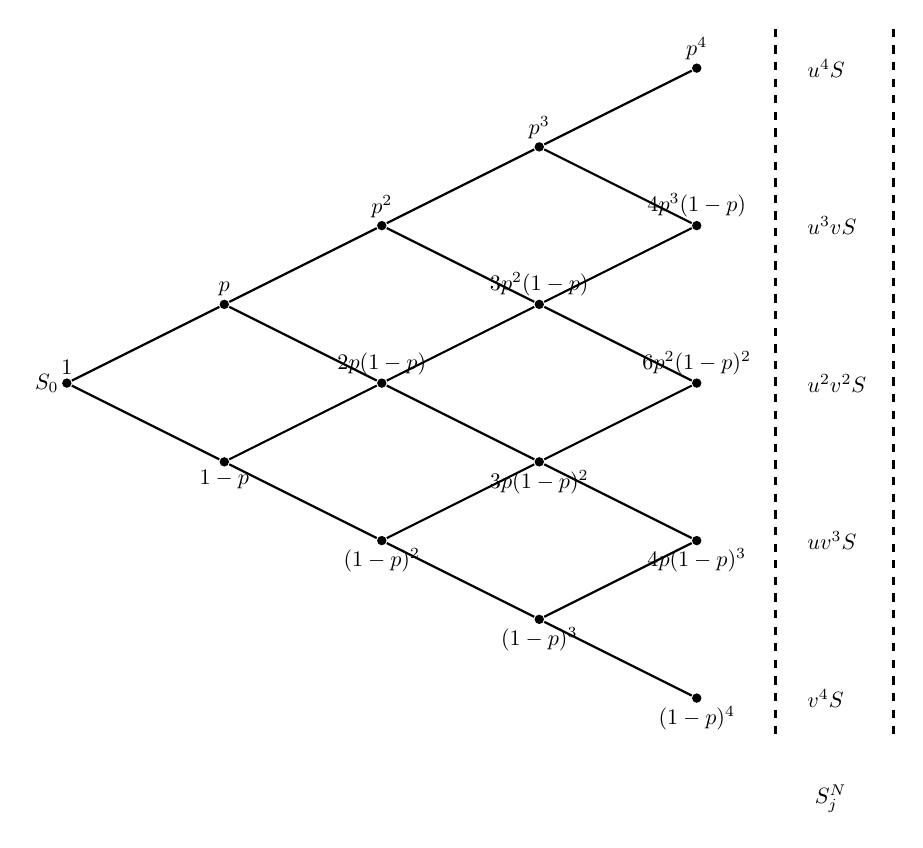
\begin{tikzpicture}[scale=1, every node/.style={scale=0.8}, every path/.style={thick}]

            % Nodes
            \node[fill=black, circle, inner sep=1.5pt] at (0,0) (N0) {};
            \node[fill=black, circle, inner sep=1.5pt] at (2,1) (N11) {};
            \node[fill=black, circle, inner sep=1.5pt] at (2,-1) (N12) {};
            \node[fill=black, circle, inner sep=1.5pt] at (4,2) (N21) {};
            \node[fill=black, circle, inner sep=1.5pt] at (4,0) (N22) {};
            \node[fill=black, circle, inner sep=1.5pt] at (4,-2) (N23) {};
            \node[fill=black, circle, inner sep=1.5pt] at (6,3) (N31) {};
            \node[fill=black, circle, inner sep=1.5pt] at (6,1) (N32) {};
            \node[fill=black, circle, inner sep=1.5pt] at (6,-1) (N33) {};
            \node[fill=black, circle, inner sep=1.5pt] at (6,-3) (N34) {};
            \node[fill=black, circle, inner sep=1.5pt] at (8,4) (N41) {};
            \node[fill=black, circle, inner sep=1.5pt] at (8,2) (N42) {};
            \node[fill=black, circle, inner sep=1.5pt] at (8,0) (N43) {};
            \node[fill=black, circle, inner sep=1.5pt] at (8,-2) (N44) {};
            \node[fill=black, circle, inner sep=1.5pt] at (8,-4) (N45) {};

            % Lines
            \draw (N0) -- (N11);
            \draw (N0) -- (N12);

            \draw (N11) -- (N21);
            \draw (N11) -- (N22);
            \draw (N12) -- (N22);
            \draw (N12) -- (N23);

            \draw (N21) -- (N31);
            \draw (N21) -- (N32);
            \draw (N22) -- (N32);
            \draw (N22) -- (N33);
            \draw (N23) -- (N33);
            \draw (N23) -- (N34);

            \draw (N31) -- (N41);
            \draw (N31) -- (N42);
            \draw (N32) -- (N42);
            \draw (N32) -- (N43);
            \draw (N33) -- (N43);
            \draw (N33) -- (N44);
            \draw (N34) -- (N44);
            \draw (N34) -- (N45);

            % Labels
            \node[above] at (N0) {$1$};
            \node[left]  at (N0) {$S_0$};
            \node[above] at (N11) {$p$};
            \node[below] at (N12) {$1-p$};

            \node[above] at (N21) {$p^2$};
            \node[above] at (N22) {$2p(1-p)$};
            \node[below] at (N23) {$(1-p)^2$};

            \node[above] at (N31) {$p^3$};
            \node[above] at (N32) {$3p^2(1-p)$};
            \node[below] at (N33) {$3p(1-p)^2$};
            \node[below] at (N34) {$(1-p)^3$};

            \node[above] at (N41) {$p^4$};
            \node[above] at (N42) {$4p^3(1-p)$};
            \node[above] at (N43) {$6p^2(1-p)^2$};
            \node[below] at (N44) {$4p(1-p)^3$};
            \node[below] at (N45) {$(1-p)^4$};


            % Payoff Values
            \node[right] at (9.3,4) {$u^4S$};
            \node[right] at (9.3,2) {$u^3vS$};
            \node[right] at (9.3,0) {$u^2v^2S$};
            \node[right] at (9.3,-2) {$uv^3S$};
            \node[right] at (9.3,-4) {$v^4S$};

            % Vertical Lines
            \draw[dashed] (9,4.5) -- (9,-4.5);
            \draw[dashed] (10.5,4.5) -- (10.5,-4.5);

            % Asset Prices Label
            \node[below] at (9.7,-5) {$S^{N}_{j}$};

        \end{tikzpicture}
        \caption{Binomial Tree for Option Pricing.}
        \label{fig:binomial_tree}
    \end{figure}

    where $S^{N}_{j}$ is the price at time step N and represents the asset price at the $j$-th tree's node.

    A relation is required $u > d$ and $S^{(n)}(0) = S_0$ is the initial price.
    A discrete-time framework is considered with equidistant time steps,
    such that $\delta t = T/n$ represents the length of each period which $T$ denotes the time to maturity
    and n is the number of periods.
    The \gls{crr} model employs a recombining binomial tree,
    achieved by imposing the condition $u = 1/d$.
    This recombination property,
    where an upward movement followed by a downward movement (or vice versa) results in the same price,
    significantly reduces the computational complexity.
    Specifically, a recombining tree with $n$ time steps contains $2n+1$ nodes,
    as opposed to $2^n$ nodes in a general non-recombining binomial tree.
    This enhanced computational efficiency makes the \gls{crr} model particularly attractive for practical applications.
    Furthermore, the recombining structure facilitates the convergence of continuous-time processes,
    such as geometric Brownian motion in the limit as $\delta t \to 0$~\cite{billingsley_convergence_1999}.

    The risk-free rate is constant and assumed to be equal to $r$.
    In addition to trading this asset,
    an investor can also invest in a back account with a continuously compounded interest rate $r$.
    Considering continuous compounding, the value of the back account grows by the factor $e^{r\delta t}$ in each period.
    The no-arbitrage principle implies that

    \begin{equation}
        u > e^{r\delta t} > d
        \label{eq:no_arbitrage_ud}
    \end{equation}

    If the above relation is violated, one can generate money without investing their own funds by either
    selling the stock short $ u < e^{r \delta t}$ or
    financing a stock purchase by a credit (in the case of $d > e^{r \delta t} $).

    The binomial method can therefore be applied as a discrete time numerical valuation of options,
    as an approximation to the Black-Scholes model.
    It is required that $p$ be chosen such that the first and second moment of the one-period log-returns is preserved,
    so that the binomial stock price framework approximates Black-Scholes.
    The parameter specification initially suggested made by \gls{crr} was

   \begin{equation}
        u = e^{\sigma \sqrt{\Delta t}}, \quad
        d = \frac{1}{u}, \quad
        p = \frac{1}{2} \left( 1 + \left( r - \frac{1}{2} \sigma^2 \right) \frac{1}{\sigma} \sqrt{\Delta t} \right)
        \label{eq:crr_parameters}
   \end{equation}

    note that the parameter $u=e^{\sigma \sqrt{\delta t}}$ comes from the need to match the variance of the
    binomial model to that of the Black-Scholes lognomal underlying price process.
    This methodology provides a closed-form expression for $u$, $d$ and $p$,
    making its implementations straightforward and computationally efficient. \\

    To implicitly include both the drift and volatility in the binomial model,
    Wilmott~\cite{wilmott_paul_2007} derives parameters $u$, $d$ and $p$ to allow more flexibility in adjusting
    for approximations or alternative assumptions.\ Despite slight differences,
    both methods follow the same principles of a lognormal underlying price process, risk-neutral valuation,
    moment matching and both require $\delta t$ to be small enough to ensure convergence to the Black-Scholes model.

    \begin{equation}
        puS + (1 - p)dS =
            SE \left[ e^{\left(\mu -\frac{1}{2} \sigma^2 \right) \delta t + \sigma \phi \sqrt{\delta t}} \right] =
            S e^{\mu \, \delta t}
        \label{eq:pw_drift}
    \end{equation}

    where $\phi$ is the standard normal random variable $\phi \sim N(0,1)$.
    Taking the expectation of S in the Black-Scholes model, we have

    \begin{equation}
        pu + (1 - p)d = e^{\mu \ \delta t}
        \label{eq:pw_s_expectation]}
    \end{equation}

    Rearranging equation~\ref{eq:pw_s_expectation]}

    \begin{equation}
        p = \frac{e^{\mu \delta t} - d}{u - d}
        \label{eq:pw_p}
    \end{equation}

    The probability $p$ here is obtained by matching the expectation of the binomial random walk with the expected
    value of the stochastic geometric Brownian motion as the underlying price process. \\

    For the binomial walk, to have the correct variance, we have again to match the variance of the binomial model
    with that of the Black-Scholes lognormal underlying price process.
    The variance is defined as $V[x] = E(x^2) - E(x)^2$.
    For both the lognormal process and the binomial walk, the variance can be expressed as follows:

    \begin{align}
        V[S] &= e^{(2\mu + \sigma^2)\delta t} - \left(e^{\mu \delta t}\right)^2 \\
        V[BinWalk] &= p u^2 + (1 - p) d^2 - \left(p u + (1 - p) d\right)^2
        \label{eq:pw_variance}
    \end{align}

    Then, from the equations~\ref{eq:pw_variance} above

    \begin{equation}
        p u^2 + (1 - p) d^2 = e^{(2\mu + \sigma^2)\delta t}
        \label{eq:pw_bw_variance}
    \end{equation}

    Using the relation to ensure node recombination $u = 1/d$, together with the equations
    ~\ref{eq:pw_p} and~\ref{eq:pw_bw_variance}, we can get the following expression for the upward factor $u$:

    \begin{equation}
        u = \frac{1}{2} \left( e^{-\mu \delta t} + e^{(\mu + \sigma^2)\delta t} \right)
            + \frac{1}{2} \sqrt{\left( e^{-\mu \delta t} + e^{(\mu + \sigma^2)\delta t} \right)^2 - 4}
        \label{eq:pw_u}
    \end{equation}

    \subsection{Binomial Option Pricing}
        \label{sec:bin_option_pricing}

    An option is a financial derivative that provides the holder with the right, but not the obligation,
    to either purchase or sell an underlying asset at a predetermined price, referred to as the strike price,
    denoted by $K$.
    The options that can only be exercised at the expiration date are known as European options,
    while those that can be exercised at any time before the expiration date are referred to as American options.
    Options are categorized into two types:
    \begin{itemize}
        \item \textbf{Call Option}: Grants the holder the right to purchase the underlying asset. \\
        The payoff is: \( \max(S_T - K, 0) \)
        \item \textbf{Put Option}: Grants the holder the right to sell the underlying asset. \\
        The payoff is: \( \max(K - S_T, 0) \)
    \end{itemize}

    The no-arbitrage principle can be extended to a generalized framework by considering a stock with an initial price
    $S_0$ and an associated option (or any derivative dependent on the stock) with a current value of $V$.
    If the stock price rises to $S_0 u$, the option's payoff is $V_u$, and if the stock price falls to $S_0 d$,
    the option's payoff is $V_d$.

    To analyze the pricing, we construct a portfolio consisting of one option and short position in a quantity $\Delta$
    of the underlying.
    The value of $\Delta$ is derived such that the portfolio becomes risk-neutral.
    A risk-free portfolio means that the value of the portfolio is the same regardless of whether
    the stock price moves up or down.
    To achieve this, we set the values of the portfolio equal in the two scenarios:

    \begin{equation}
        S_0 u \Delta- V_u = S_0 d \Delta - V_d
        \label{eq:risk_neutral}
    \end{equation}

    this means the amount of $\Delta$ should be

    \begin{equation}
        \Delta = \frac{V_u - V_d}{(u - d) S_0}
        \label{eq:delta}
    \end{equation}

    In this case, the portfolio is risk-less and, for there to be no arbitrage opportunities,
    it must earn the risk-free interest rate.
    Equation~\ref{eq:delta} shows that $\Delta$ is the ratio of the change in the option price to the change
    in the stock price as we move between the nodes at time $T$.

    By the no-arbitrage principle, the cost of setting up the portfolio must be equal to the present value of the portfolio.

    \begin{equation}
        S_0 \Delta - V = (S_0 u \Delta - V_u)e^{-rT}
        \label{eq:no_arbitrage}
    \end{equation}

    If we denote the risk-free interest rate by $r$ for the present value,
    assuming continuous discounting $e^{-rT}$.
    Rearrange the equation to get the option value $V$ and substitute $\Delta$ from equation~\ref{eq:delta}

    \begin{equation}
        V = e^{-rT} [p V_u + (1 - p) V_d]
        \label{eq:option_value}
    \end{equation}

    where

    \begin{equation}
        p = \frac{e^{rT} - d}{u - d}
        \label{eq:prob_value}
    \end{equation}

    American-style exercise can be effectively implemented within a binomial framework.
    Consider dividing the life of an American option into $N$ intervals, each of length $\Delta t$.
    The $j$th node at time $i \Delta t$ will be denoted as the $(i, j)$ node,
    where $0 \leq i \leq N$ and $0 \leq j \leq i$.
    Let $V_{i,j}$ represent the value of the option at the $(i, j)$ node.
    The underlying asset price at the $(i, j)$ node is given by $S_0 u^j d^{i-j}$.
    For a call option, its value at time $T$ (the expiration date) is expressed as

    \begin{equation}
        V_{N,j} = \max
            \left\lbrace
                S_0 u^j d^{N-j} - K, 0
            \right\rbrace, \quad j = 0, 1, \ldots, N
        \label{eq:call_option}
    \end{equation}

    As presented in~\ref{fig:binomial_tree},
    there is a probability $p$ of moving from the $(i, j)$ node at time $i \delta t$ to the $(i+1, j+1)$
    node at time $(i+1) \delta t$, and a probability $1 - p$ of moving from the $(i, j)$ node at
    time $i \delta t$ to the $(i+1, j)$ node at time $(i+1) \delta t$.
    Assuming no early exercise (European), a risk-neutral valuation gives:

    \begin{equation}
        V_{i,j} = e^{-r \Delta t} \left[ p V_{i+1, j+1} + (1 - p) V_{i+1, j} \right]
        \label{eq:european_option}
    \end{equation}

    for $0 \leq i \leq N-1$ and $0 \leq j \leq i$.
    To take account of early exercise (American),
    this value for $V_{i,j}$ must be compared with the option's intrinsic value, so that for a call:

    \begin{equation}
        V_{i,j} = \max
            \left\lbrace
                S_0 u^j d^{i-j} - K, \, e^{-r \Delta t} \left[ p V_{i+1, j+1} + (1 - p) V_{i+1, j} \right]
            \right\rbrace
        \label{eq:american_call_option}
    \end{equation}

    The primary distinction between European and American option pricing lies in the ability to exercise
    an American option at any point prior to expiration.
    Consequently, at each node in the pricing model,
    the value of the option must be compared to its intrinsic value to determine whether early exercise is optimal.

    Below is a Python code snippet that implements the binomial option pricing model for the American option.
    The European option is also implemented in the same way, using equation~\ref{eq:european_option} instead.
    To implement the model efficiently, the code uses the NumPy library and operations are fully vectorized.
    Due the recursive nature of the model, the code uses a backward induction approach to calculate the option price.

    \begin{lstlisting}[
       language=Python,
       caption={Python Code: American option price},
       label={lst:american_option_price}
    ]
import numpy as np


def binomial_recomb_uptriang(a, n):
    # Create a grid of indices for powers
    rows, cols = np.triu_indices(n + 1)

    # Compute terms for (a + 1/a)^n
    terms = a ** ((cols - rows) + (np.sort(rows - cols)[::-1]))

    # Create an upper diagonal matrix
    matrix = np.zeros((n + 1,  n + 1))
    matrix[rows, cols] = terms
    return  matrix


def american_option_price(S0, sigma, r, K, T, N, option_type):
    # Time step
    dt = T / N

    # Discount factor
    disc = np.exp(-r * dt)

    # Up and down factors
    temp1 = np.exp((r + sigma ** 2) * dt)
    temp2 = 0.5 * (temp1 + disc)
    u = temp2 + np.sqrt(temp2 ** 2  - 1)
    d = 1 / u

    # Probability
    p = (np.exp(r * dt) - d) / (u - d)

    # Generate stock prices
    S = S0 * binomial_recomb_uptriang(u, N)

    # Calculate payoff based on option type
    payoff = (S - K) if option_type == "call" else (K - S)
    opt_val = np.maximum(payoff, 0)

    # Initialize option values at maturity
    V = np.zeros((N + 1, N + 1))
    V[:,-1] = opt_val[:,-1]

    # Backward induction through the tree
    for n in range(N):
        col=N-n
        # Calculate the discounted value
        disc_value = (p * V[:col, col] + (1 - p) * V[1 : col+1, col]) * disc

        # Update option values
        V[:col, col-1] = np.maximum(disc_value, opt_val[:col, col-1])
    return V
   \end{lstlisting}

\section{Continuous-Time Modelling: Black-Scholes Closed Form}
    \label{sec:cont_time}

    The Black-Scholes model, introduced in 1973 by Fischer Black and Myron Scholes,
    transformed the field of quantitative finance by providing a rigorous mathematical framework for
    pricing European-style options~\cite{black_pricing_1973}.
    The model derives theoretical estimates of option prices based on a set of key factors and
    assumptions~\cite{wilmott_paul_2007}:

    \enumerate{
        \item The underlying asset follows a lognormal stochastic process
        \item The risk-free interest rate is a known function of time
        \item There are no dividends paid on the underlying asset
        \item There are no transaction costs or taxes
        \item Delta hedging is done continuously
        \item The market is frictionless, with no arbitrage opportunities
        \label{itm:bs_assumptions}
    }

    The reasoning underlying the equation, in essence, parallels to the methodology applied in
    the binomial lattice~\ref{sec:desc_time}.
    At every discrete time step, a selection of two obtainable financial instruments is performed,
    which guides the assembly of a portfolio.
    The design of this portfolio is such that it emulates the local dynamics of the derivative security. \\

    Let the price $S$ denote the underlying security be governed by a geometric Brownian motion process
    over a time interval $[0, T]$ described by the stochastic differential equation:

    \begin{equation}
        dS = \mu S dt + \sigma S dW
        \label{eq:geometric_brownian}
    \end{equation}

    where $\mu$ is the drift rate (expected return), $\sigma$ is the volatility and $W$ is a
    standard Wiener process.

    Using $\Pi$ to represent the portfolio value, the Black-Scholes model is derived by constructing a
    long option position and a short position in the underlying asset in some quantity $\Delta$,
    similar to what was donein the binomial model~\ref{eq:risk_neutral}:

    \begin{equation}
        \Pi = V(S,t) - \Delta S
        \label{eq:portfolio_value}
    \end{equation}

    Therefore, it can be surmised that the fluctuations in the portfolio's value can be attributed to the temporal
    changes in the option's value and its underlying asset.

    \begin{equation}
        d\Pi = dV - \Delta dS
        \label{eq:portfolio_fluctuation}
    \end{equation}

    Applying Itô's lemma to the option value $V(S,t)$~\cite{kuo_introduction_2006}, we have

    \begin{gather}
        \begin{split}
            dS(t)
                = g(S,t) dt + f(S,t) dW(t) \\
        \end{split}
        \label{eq:itos_process}
            \\
        \begin{split}
            dV(S, t)
                =
                    \left(
                        \frac{\partial V}{\partial t}
                        + \frac{\partial V}{\partial S} g(S,t)
                        + \frac{1}{2} \frac{\partial^2 V}{\partial S^2} f(S,t)^2
                    \right) dt
                    + \frac{\partial V}{\partial S} f(t) dW(t)
        \end{split}
        \label{eq:itos_lemma}
            \\
        \begin{split}
            g(S,t) = \mu S, \quad f(S,t) = \sigma S
        \end{split}
        \label{eq:itos_functionals}
    \end{gather}

    applying eq.~\ref{eq:itos_functionals} into eq.~\ref{eq:itos_lemma} we have

    \begin{equation}
        dV =
            \left(
                \frac{\partial V}{\partial t}
                    + \frac{\partial V}{\partial S} \mu S
                    + \frac{1}{2} \frac{\partial^2 V}{\partial S^2} \sigma^2 S^2
            \right) dt
            + \frac{\partial V}{\partial S} \sigma S dW
        \label{eq:itos_bs}
    \end{equation}

    Observe that the component situated within the parentheses, whose value is contingent upon $dt$,
    is deterministic in nature.
    The stochastic part of the equation is the last term,
    which is the product of the option's delta and the Wiener process.

    Substituting eq.~\ref{eq:itos_bs} into eq.~\ref{eq:portfolio_fluctuation} we have

    \begin{equation}
        d\Pi =
            \left(
                \frac{\partial V}{\partial t}
                    + \frac{\partial V}{\partial S} \mu S
                    + \frac{1}{2} \frac{\partial^2 V}{\partial S^2} \sigma^2 S^2
            \right) dt
            + \frac{\partial V}{\partial S} \sigma S dW
            - \Delta dS
        \label{eq:portfolio_fluctuation_bs}
    \end{equation}

    now including back the underlying asset price $S$~eq.\ref{eq:geometric_brownian} we have

    \begin{equation}
        d\Pi =
            \left(
                \frac{\partial V}{\partial t}
                    + \frac{\partial V}{\partial S} \mu S
                    + \frac{1}{2} \frac{\partial^2 V}{\partial S^2} \sigma^2 S^2
            \right) dt
            + \frac{\partial V}{\partial S} \sigma S dW
            - \Delta \left( \mu S dt + \sigma S dW \right)
        \label{eq:portfolio_fluctuation_bs_s}
    \end{equation}

    To eliminate the stochastic term, the parameter $\Delta$ is chosen such that the coefficient of $dW$ is zero.
    This condition is known as the delta-hedging strategy, which ensures that the portfolio is risk-free.
    Delta hedging is an example of a dynamic hedging strategy.
    From one time step to the next the quantity $\frac{\partial V}{\partial S}$ changes, since it is, like V,
    a function of the ever-changing variablesS and t.
    This means that the perfect hedge must be continually rebalanced.
    Choosing carefully the quantity $\Delta$ we have

    \begin{equation}
        \Delta = \frac{\partial V}{\partial S}
        \label{eq:delta_hedge}
    \end{equation}

    Substituting eq.~\ref{eq:delta_hedge} into eq.~\ref{eq:portfolio_fluctuation_bs_s} we have

    \begin{equation}
        d\Pi =
            \left(
                \frac{\partial V}{\partial t}
                + \frac{1}{2} \frac{\partial^2 V}{\partial S^2} \sigma^2 S^2
            \right) dt
        \label{eq:portfolio_fluctuation_bs_s_delta}
    \end{equation}

    With respect to the delta-hedging strategy implemented, the term $\frac{\partial V}{\partial S} \mu S dt$ dissipates.
    This approach ascertains a risk-free portfolio by concurrently eliminating both the stochastic and drift terms.
    From an economic perspective, the rationale behind this phenomenon is anchored on the risk elimination
    brought about by a perfect hedge using the underlying asset.
    As such, there is no reward corresponding to unnecessary risk exposure.
    Only the risk-free rate of return is incorporated in the equation.
    This fundamental principle implies that with a mutual agreement on an asset's volatility,
    there is a likelihood of agreeing on the valuation of its derivatives,
    despite possible deviations in the estimates of the drift.  \\

    Examining the implications of eq.~\ref{eq:portfolio_fluctuation_bs_s_delta} culminates in the derivation that
    it is entirely devoid of risk.
    An invariable change in the portfolio value, denoted as $\Pi$, which is risk-free, should align coherently with
    the appreciation derived from investing an equivalent amount of capital in a risk-free interest-bearing account:

    \begin{equation}
        d\Pi = r \Pi dt
        \label{eq:risk_free}
    \end{equation}

    Substituting into eq.~\ref{eq:portfolio_fluctuation_bs_s_delta} eq.~\ref{eq:risk_free}, taking into account the
    portfolio value $\Pi$ from eq.~\ref{eq:portfolio_value} and $\Delta$~\ref{eq:delta_hedge}, we have:

    \begin{equation}
        \left(
            \frac{\partial V}{\partial t}
            + \frac{1}{2} \frac{\partial^2 V}{\partial S^2} \sigma^2 S^2
        \right) dt
        = r \left( V - \frac{\partial V}{\partial S} S \right) dt
        \label{eq:portfolio_fluctuation_bs_s_delta_r}
    \end{equation}

    Rearranging the terms in eq.~\ref{eq:portfolio_fluctuation_bs_s_delta_r} we have the Black-Scholes partial
    differential equation:

    \begin{equation}
        \frac{\partial V}{\partial t}
        + \frac{1}{2} \frac{\partial^2 V}{\partial S^2} \sigma^2 S^2
        + r S \frac{\partial V}{\partial S}
        - r V = 0
        \label{eq:black_scholes}
    \end{equation}

    To solve this partial differential equation, the Black-Scholes model requires the specification of the option's
    boundary conditions.
    For a European call option, the boundary conditions are:
    \begin{itemize}
        \item At \textbf{$T$}: the option's value is the payoff: $V(S, T) = \max(S - K, 0)$
        \item As \textbf{$S \to 0$}: the option's value approaches zero: $V(0, t) = 0$
        \item As \textbf{$S \to \infty$}: the option's value approaches the stock price:
            $V(S, t) \approx S - Ke^{-r\left( T-t \right)}$
        \label{eq:boundary_conditions}
    \end{itemize}

    The Black-Scholes eq.~\ref{eq:black_scholes} can be accurately interpreted as a reaction-convection-diffusion
    equation. It is a parabolic partial differential equation, meaning that it is a second-order derivative with respect
    to the underlying asset price $S$ and first-order derivative with respect to time $t$.
    Equations of this type are commonly used in physics to model phenomena such as heat conduction and diffusion.
    Making a close analogy to the heat equation, its terms can be interpreted as follows:

    \begin{itemize}
        \item $\frac{\partial V}{\partial t}$: represents the option's time decay
        \item $\frac{1}{2} \frac{\partial^2 V}{\partial S^2} \sigma^2 S^2$:
        diffusion component, which quantifies of the inherent volatility in the price of the option.
        \item $r S \frac{\partial V}{\partial S}$: is the convection term, which accounts for the option's drift
        \item $r V$: is the reaction term, which describes for the risk-free interest rate
        \label{eq:bs_terms}
    \end{itemize}

    The strategy for solving the Black-Scholes equation is to transform it into a heat equation,
    which is a well-known partial differential equation with a known solution.


    We start by switching from the present value of the option to a future value perspective.
    Since the payoff takes place at time $T$ but we are valuing it at the earlier time $t$,
    we introduce a varible $\tau = T - t$, since we are solving the equation backwards in time.
    Defining the derivative value function $V(S,t)$, as the present value of the option to future value terms:

    \begin{equation}
        V(S,\tau) = e^{-r \tau},U(S,\tau)
        \label{eq:future_val}
    \end{equation}

    Substituting eq.~\ref{eq:future_val} into eq.~\ref{eq:black_scholes} and rearranging the terms to have:

    \begin{equation}
        \frac{\partial U}{\partial \tau}
        = \frac{1}{2} \sigma^2 \frac{\partial^2 U}{\partial S^2}
        + rS \frac{\partial U}{\partial S}
        \label{eq:heat_eq}
    \end{equation}

    Since stock prices often follow a log-normal process, we define $z = ln(S)$.
    This change of variables yields the following derivatives:

    \begin{equation*}
        \begin{aligned}
            \frac{\partial}{\partial S} &= e^{-z}\,\frac{\partial}{\partial z}
        \end{aligned}
        \qquad
        \begin{aligned}
            \frac{\partial^2}{\partial S^2} &= e^{-2z}\,\frac{\partial^2}{\partial z^2}
            - e^{-2z}\,\frac{\partial}{\partial z}
        \end{aligned}
    \end{equation*}

    Substituting these derivatives into eq.~\ref{eq:heat_eq}, we have:

    \begin{equation}
        \frac{\partial U}{\partial \tau} =
        \frac{1}{2} \sigma^2 \frac{\partial^2 U}{\partial z^2}
        + \left( r - \frac{1}{2} \sigma^2 \right) \frac{\partial U}{\partial z}
        \label{eq:heat_eq_z}
    \end{equation}

    We have thus recast the problem from 0 < S < $\infty$ (S is log-normal) to $-\infty$ < z < $\infty$. Moreover,
    all coefficients in eq.~\ref{eq:heat_eq_z} are constant, which makes it a linear partial differential equation.

    Finally, we define $U = u(x, \tau)$ and perform a shift in the $(z,\tau)$ coordinate system:

    \begin{equation}
        x = z + \left( r - \frac{1}{2} \sigma^2 \right) \tau
        \label{eq:shift}
    \end{equation}

    This translation is analogous to using a forward price in place of the spot price.
    Under this change of variables~\ref{eq:shift},
    the Black-Scholes equation becomes the diffusion equation which has a known solution.

    \begin{equation}
        \frac{\partial u}{\partial \tau} = \frac{1}{2} \sigma^2 \frac{\partial^2 u}{\partial x^2}
        \label{eq:diffusion_eq}
    \end{equation}

    The exact solution, applying the boundary conditions defined in~\ref{eq:boundary_conditions},
    ~\cite{wilmott_paul_2007}, is given by the solution in the integral form:

    \begin{equation}
        V(S,t) =
            \frac{e^{-r(T-t)}}{\sigma \sqrt{2 \pi (T-t)}}
            \int_{0}^{\infty} e^{-\frac{1}{2}\left(
                 \frac{\log(S/S') + (r - \frac{1}{2}\sigma^2)(T-t)}{\sigma \sqrt{T-t}}
            \right)^2}
            \text{Payoff}(S') \frac{dS'}{S'}
        \label{eq:bs_solution_integral}
    \end{equation}

    where x' = log(S') and Payoff(S') is the payoff function of the option at expiration.

    The payoff function for a European call option can be expressed as $max(S - K, 0)$.
    Substituting this into the integral representation for the option price yields integrals involving $S$ and $K$
    that can be rewritten in the form

    \begin{equation}
        \int_{d}^{\infty} e^{-\tfrac{1}{2} x^2} \,\frac{dx}{x}
            \longrightarrow
            N(x) = \int_{-\infty}^{x} e^{-\tfrac{1}{2} \phi^2} d\phi
        \label{eq:form_integral}
    \end{equation}

    illustrating how these terms relate to the standard Normal cumulative distribution function.
    Thus, the Black-Scholes model provides a closed-form solution for European options can be elegantly expressed:

    \begin{equation}
        C(S,t) = S N(d_1) - K e^{-r(T-t)} N(d_2)
        \label{eq:bs_solution}
    \end{equation}

    where

    \begin{equation}
        \begin{aligned}
            d_1 &= \frac{\log(S/K) + (r + \tfrac{1}{2}\sigma^2)(T-t)}{\sigma \sqrt{T-t}} \\
            d_2 &= d_1 - \sigma \sqrt{T-t}
        \end{aligned}
        \label{eq:bs_d1_d2}
    \end{equation}

    To demonstrate a practical application of the Black--Scholes model for pricing call options,
    we now consider a delta-hedged short call position.
    One begins by assuming that the underlying asset is overvalued, intending to profit from the high option premium.
    This position consists of two main components:
    selling the call option and simultaneously purchasing a fraction (the delta) of the underlying asset.
    The fraction purchased serves to hedge against adverse movements in the option’s price.

    In this example, we construct what is termed a self-financing portfolio, meaning that there is
    no initial net cash outflow. Specifically, the premium received from the sale of the call option
    is used in conjunction with borrowing at the risk-free rate to acquire the delta amount of the
    underlying asset. For simplicity, we do not incorporate rebalancing, which in a more general
    treatment would involve continuously adjusting the delta-hedged position to maintain an effective hedge.
    This lack of rebalancing is a notable simplification, as the Black-Scholes framework typically assumes
    the ability to rebalance continuously throughout the life of the option.
    The three main components of the position are:

    \begin{itemize}
        \item Short 1 call option: The premium received from selling the call option
        \item Buy delta shares: The cost of purchasing the delta amount of the underlying asset
        \item Borrow cash: The amount borrowed to net the initial cash flow to zero
        \label{eq:position_components}
    \end{itemize}

    Below is a Python code snippet that demonstrates a delta-hedged short call position using the Black-Scholes model.
    The code calculates the call price and delta using the Black-Scholes formula, sets up the position under the
    following assumptions:

    \begin{itemize}
        \item Underlying price (S0) = \$100
        \item Strike (K) = \$100
        \item Time to maturity (T) = 1 year
        \item Risk-free rate (r) = 5\%
        \item Volatility (sigma) = 25\%
        \item Terminal stock prices at maturity: \$90 and \$120
        \label{eq:position_setup}
    \end{itemize}

    where for each terminal stock price ($[S < K ,S > K]$), the final payoff is calculated,
    ignoring continuous rebalancing.
    In practice, the delta of a call option can be computed using the Black-Scholes formula
    ~\cite{luenberger_investment_2014}:

    \begin{equation}
        \Delta = N(d_1)
        \label{eq:delta_bs}
    \end{equation}

    where $N$ is the standard normal cumulative distribution function and $d_1$ is given by eq.~\ref{eq:bs_d1_d2}.

    \begin{lstlisting}[
       language=Python,
       caption={Python Code: Delta hedge short call example},
       label={lst:delta_hedged_short_call}
    ]
import numpy as np
from scipy.stats import norm

def black_scholes_call(
    S: float,    # Underlying price
    K: float,    # Strike price
    T: float,    # Time to maturity
    r: float,    # Risk-free rate
    sigma: float # Volatility
) -> tuple[float, float]:

    # d1 and d2
    d1 = (np.log(S / K) + (r + 0.5 * sigma**2) * T) / (sigma * np.sqrt(T))
    d2 = d1 - sigma * np.sqrt(T)

    # Call price
    call_price = S * norm.cdf(d1) - K * np.exp(-r * T) * norm.cdf(d2)

    # Delta
    delta_call = norm.cdf(d1)

    return call_price, delta_call

def delta_hedged_short_call_example(S, K, T, r, sigma, terminal_prices):

    # Demonstrates a delta-hedged short call using:
    #  - The short call option
    #  - A delta hedge in the underlying
    #  - A risk-free borrowing/lending position
    #
    # It sets up the position,\so the initial net cash flow is zero,
    # then calculates the final P&L at two potential stock prices at maturity
    # and ignoring continuous balancing.

    # 1) Compute call price and delta using Black-Scholes
    call_price, delta_call = black_scholes_call(S, K, T, r, sigma)

    print("=== Black-Scholes Computations ===")
    print(f"Underlying price (S0) = {S:.2f}")
    print(f"Strike (K)            = {K:.2f}")
    print(f"Time to maturity (T)  = {T:.2f} year(s)")
    print(f"Risk-free rate (r)    = {r:.2%}")
    print(f"Volatility (sigma)    = {sigma:.2%}\n")
    print(f"Call Price = ${call_price:.2f}")
    print(f"Call Delta = {delta_call:.3f}\n")

    # 2) Set up the delta-hedged short call

    # Short 1 call => collect premium
    premium_received = call_price

    # Buy delta_call shares => negative cashflow
    cost_shares = delta_call * S

    # Borrow the difference so initial net = 0
    borrowed = cost_shares - premium_received

    print("=== Position Setup (Initial) ===")
    print(f"Short 1 call: +${premium_received:.2f} premium")
    print(f"Buy {delta_call:.3f} shares: -${cost_shares:.2f}")
    print(f"""Borrow cash:
        +${borrowed:.2f} (to net initial cashflow to $0.00)\n""")

    # 3) Evaluate final payoff for two terminal prices
    #    ignoring continuous rebalancing

    print("=== Payoff at Expiry (Discrete, No Rebalancing or Interest) ===")
    for S_T in terminal_prices:
        # Short call payoff: -(max(S_T - K, 0)) #plus the call premium
        call_exercise_value = max(S_T - K, 0.0)
        short_call_pnl = premium_received - call_exercise_value

        # Stock payoff: final stock value minus what we paid at inception
        stock_final_value = delta_call * S_T
        stock_pnl = stock_final_value - cost_shares

        # Bond/cash payoff: we owe exactly the borrowed amount
        # (ignoring interest)
        bond_pnl = borrowed - borrowed * (1+r)**T

        total_pnl = short_call_pnl + stock_pnl + bond_pnl

        print(f"Final Stock Price: S_T = ${S_T:.2f}")
        print(f"  - Short Call P&L  = ${short_call_pnl:.2f}")
        print(f"  - Stock P&L       = ${stock_pnl:.2f}")
        print(f"  - Bond (Borrowed) = ${bond_pnl:.2f}")
        print(f"  --> TOTAL P&L     = ${total_pnl:.2f}\n")


delta_hedged_short_call_example(
    S=100.0,
    K=100.0,
    T=1.0,
    r=0.05,
    sigma=0.25,
    term_prices=[90.0, 120.0]
)
# === Black-Scholes Computations ===
Call Price = $12.34
Call Delta = 0.627

# === Position Setup (Initial) ===
Short 1 call: +$12.34 premium
Buy 0.627 shares: -$62.74
Borrow cash: +$50.40 (to net initial cashflow to $0.00)

# === Payoff at Expiry (Discrete, No Rebalancing or Interest) ===
# Final Stock Price: S_T = $90.00
  - Short Call P&L  = $12.34
  - Stock P&L       = $-6.27
  - Bond (Borrowed) = $-2.52
  --> TOTAL P&L     = $3.54

# Final Stock Price: S_T = $120.00
  - Short Call P&L  = $-7.66
  - Stock P&L       = $12.55
  - Bond (Borrowed) = $-2.52
  --> TOTAL P&L     = $2.36

   \end{lstlisting}

    Final net P\&L from the three positions ends up very close to $0$,
    apart from small differences due to ignoring that Delta would actually change as the stock price moved.
    In an ideal Black–Scholes world with continuous rebalancing,
    the result would hedge out the stock’s movements perfectly,
    and your profit (if any) would come from the option’s implied volatility being overpriced compared to
    realised volatility.

\section{Numerical Methods: Black-Scholes PDE}
    \label{sec:pde}

    In many practical scenarios, deriving closed-form expressions for option valuations proves
    to be challenging. Consequently, it becomes necessary to approach these problems using
    numerical techniques. One commonly studied approach is the binomial method, see section~\ref{sec:desc_time},
    in which a finite tree structure is constructed to model the evolution of the underlying asset price
    from the current time until the expiry date. The binomial method may be interpreted as
    a specialized technique for discretizing a partial differential equation. Its generalization
    lies in finite-difference methods, where grids and meshes replace the notion of trees.

    When transforming a differential equation (e.g Black–Scholes equation) into
    a difference equation, it is often more convenient to use a uniform grid rather than a
    tree structure. This approach simplifies the process, and there exist numerous enhancements
    that can improve both the efficiency and accuracy of the finite-difference method. In contrast,
    the binomial method is less flexible regarding modifications.

    One fundamental difference between binomial and finite-difference methods is how
    diffusion (i.e., volatility) is represented. In the binomial approach, the diffusion is
    embedded within the branching structure. By contrast, finite-difference methods fix the
    underlying mesh and instead adjust certain parameters to capture changing diffusion
    dynamics~\cite{wilmott_paul_2006}.

    Using a finite-difference method, we need to define the domain of the problem,
    going from continuous $D = \left\{S_{min} < S < S_{max}; 0 < \tau < T \right\}$ to a discrete grid.
    Since a geometric Brownian motion stochastic process is assumed for the underlying, $S$ is log-normally distributed,
    hence $S_{min} = 0$.

    \begin{equation}
        D =
            \begin{cases}
                S_i = i \delta S,   \delta S = \frac{S_{max}}{M},   i = 0, 1, \ldots, M \\
                t_k = T - k \delta t,   \delta t = \frac{T}{N}, k = 0, 1, \ldots, N \\
                V_{i}^{k} = V(S_i, t_k)
            \end{cases}
        \label{eq:grid_domain}
    \end{equation}

    where the grid is descritized by the number of points in the stock price dimension $M$
    and the number of points in the time dimension $N$.

    The Black-Scholes partial differential equation~\ref{eq:black_scholes} previously derived can be discretized
    using a finite-difference method.
    Applying it to the space state varibles we can easily compute the Greeks~\cite{hirsa_computational_2024}:

    \begin{itemize}
        \item Delta ($\Delta$):
            \begin{equation}
                \Delta \approx \frac{V_{j+1}^{m} - V_{j-1}^{m}}{2\Delta S}.
                \label{eq:greek_delta}
            \end{equation}

        \item Gamma ($\Gamma$):
            \begin{equation}
                \Gamma \approx \frac{V_{j+1}^{m} - 2V_{j}^{m} + V_{j-1}^{m}}{(\Delta S)^{2}}
                \label{eq:greek_gamma}
            \end{equation}
    \end{itemize}

    The Delta was computed using the central difference method, which is a second-order accurate approximation,
    whereas the Gamma comes from a Taylor series expansion of the Delta.
    Both approximations have an error of the order $O(\Delta S^2)$~\cite{wilmott_paul_2006}.
    With regards to the spacial discretization, the Black-Scholes equation can be approximated, substituting the
    Delta and Gamma approximations, as follows:

    \begin{equation}
        a_{j} \left( V_{j+1}^{m} - 2V_{j}^{m} + V_{j-1}^{m} \right)
        + b_{j} \left( V_{j+1}^{m} - V_{j-1}^{m} \right)
        + c_{j} V_{j}^{m}
        \label{eq:spacial_discretization}
    \end{equation}

    where the coefficients $a_{j}$, $b_{j}$, and $c_{j}$ are given by:

    \begin{equation}
            a_j = \frac{\sigma^2 S_{j}^2}{2(\Delta S)^2},  \qquad
            b_j = \frac{r S_j}{2 \Delta S}, \qquad
            c_j = -r
        \label{eq:coefficients}
    \end{equation}

    The time discretization is mostly performed using a first-order accurate approximation. There three main schemes
    used in the literature: explicit, implicit methods and combination of both, the Crank-Nicolson method.

    \subsection{Explicit (Forward-Time, Central-Space)}
    \label{sec:explicit}

    In the explicit scheme, we use the forward difference in time to compute (the Greek $\theta$):

    \begin{equation}
        \theta = \frac{\partial V}{\partial t} \approx \frac{V_j^{m+1} - V_j^m}{\Delta t}
        \label{eq:forward_diff}
    \end{equation}

    Hence, from the Black-Scholes PDE:

    \begin{equation}
        \frac{V_j^{m+1} - V_j^m}{\Delta t} =
            a_j \left(V_{j+1}^m - 2V_j^m + V_{j-1}^m\right) + b_j \left(V_{j+1}^m - V_{j-1}^m\right) + c_j V_j^m
        \label{eq:explicit_scheme}
    \end{equation}

    Rearrange to solve for $V_j^{m+1}$:

    \begin{equation}
        V_j^{m+1} =
            V_j^m
            + \Delta t \left[
                a_j \left(V_{j+1}^m - 2V_j^m + V_{j-1}^m\right)
                + b_j \left(V_{j+1}^m - V_{j-1}^m\right)
                + c_j V_j^m
            \right]
        \label{eq:explicit_scheme_rearranged}
    \end{equation}

    Now group the terms involving $V_{j-1}^m$, $V_j^m$ and $V_{j+1}^m$ on the right-hand side.
    We define:
    \begin{equation*}
        \begin{aligned}
            A_j &= \Delta t \left(a_j - b_j\right), \\
            B_j &= 1 + \Delta t \left(-2a_j + c_j\right),\\
            C_j &= \Delta t \left(a_j + b_j\right)
        \end{aligned}
        \label{eq:abc}
    \end{equation*}

    Then we can write:

    \begin{equation}
        V_j^{m+1} = A_j V_{j-1}^m + B_j V_j^m + C_j V_{j+1}^m
        \label{eq:explicit_scheme_final}
    \end{equation}

    All values $V_{j-1}^m$, $V_j^m$$V_{j+1}^m$ are known at time level $m$, so $V_j^{m+1}$ can be computed explicitly.
    We do this for $j = 1, 2, \ldots, N-1$.
    The boundary points $j = 0$ and $j = N$ are handled by boundary conditions.

    \subsection{Fully Implicit (Backward-Time, Central-Space)}
    \label{sec:implicit}

    In the fully implicit method, we use a backward difference in time:

    \begin{equation}
        \frac{\partial V}{\partial t} \approx \frac{V_j^m - V_j^{m-1}}{\Delta t}
        \label{eq:backward_diff}
    \end{equation}

    So the Black-Scholes PDE at time level $m$ (unknown) becomes:

    \begin{equation}
        \frac{V_j^m - V_j^{m-1}}{\Delta t} =
            a_j \left(V_{j+1}^m - 2V_j^m + V_{j-1}^m\right)
            + b_j \left(V_{j+1}^m - V_{j-1}^m\right)
            + c_j V_j^m
        \label{eq:implicit_scheme}
    \end{equation}

    Rearrange to group all the $V_j^m$-terms on the left side:

    \begin{equation}
        V_j^m - \Delta t \left[
            a_j \left(V_{j+1}^m - 2V_j^m + V_{j-1}^m\right)
            + b_j \left(V_{j+1}^m - V_{j-1}^m\right)
            + c_j V_j^m
        \right] = V_j^{m-1}
        \label{eq:implicit_scheme_rearranged}
    \end{equation}

    Distribute $\Delta t$ and collect like terms in $V_{j-1}^m$, $V_j^m$, and $V_{j+1}^m$.
    We get a tridiagonal system of the form:

    \begin{equation}
        -A_j V_{j-1}^m + B_j V_j^m - C_j V_{j+1}^m = V_j^{m-1}
        \label{eq:tridiagonal_system}
    \end{equation}

    where:

    \begin{equation*}
        \begin{aligned}
            A_j &= \Delta t \left(a_j - b_j\right), \\
            A_j &= 1 + \Delta t \left(2a_j - c_j\right), \\
            A_j &= \Delta t \left(a_j + b_j\right)
        \end{aligned}
        \label{eq:abc_coeffs}
    \end{equation*}

    Here the unknowns are $V_1^m, V_2^m, \ldots, V_{N-1}^m$.
    We solve this tridiagonal system at each time step $m$.
    Once solved, we move backward from $m = M$ down to $m = 0$.

    \subsection{Crank–Nicolson (CN) Method}
    \label{sec:crank_nicolson}

    The Crank–Nicolson scheme is a time-centered method often viewed as the average of the explicit and implicit methods.
    It approximates:

    \begin{equation}
        \frac{\partial V}{\partial t} \bigg|_{m+\frac{1}{2}} \approx \frac{V_j^{m+1} - V_j^m}{\Delta t}
        \label{eq:cn_approx}
    \end{equation}

    and uses the spatial derivatives evaluated at the midpoint in time, i.e.,
    \begin{equation*}
        \frac{1}{2} \left[\text{spatial derivative at } m+1 \right]
        + \frac{1}{2} \left[\text{spatial derivative at } m\right].
    \end{equation*}

    Concretely, for the Black-Scholes PDE:

    \begin{equation}
        \begin{aligned}
            \frac{V_j^{m+1} - V_j^m}{\Delta t}
            &= \frac{1}{2} \underbrace{
                \Bigl[
                a_j \bigl(V_{j+1}^{m+1} - 2V_j^{m+1} + V_{j-1}^{m+1}\bigr)
                + b_j \bigl(V_{j+1}^{m+1} - V_{j-1}^{m+1}\bigr)
                + c_j V_j^{m+1}
                \Bigr]
            }_{\text{implicit part}} \\
            &+ \underbrace{
                \Bigl[
                a_j \bigl(V_{j+1}^m - 2V_j^m + V_{j-1}^m\bigr)
                + b_j \bigl(V_{j+1}^m - V_{j-1}^m\bigr)
                + c_j V_j^m
                \Bigr]
            }_{\text{explicit part}}
        \end{aligned}
        \label{eq:cn_black_scholes}
    \end{equation}

    We then rearrange terms to get a system of the form:

    \begin{equation}
        \left[
            1 - \frac{\Delta t}{2} \left(-2a_j + c_j\right)
        \right] V_j^{m}
        + \frac{\Delta t}{2} \left(a_j + b_j\right) V_{j+1}^{m}
        + \frac{\Delta t}{2} \left(a_j - b_j\right) V_{j-1}^{m}
        \propto V^{m+1}
        \label{eq:cn_rearranged}
    \end{equation}

    But more commonly, we place all $m+1$-terms on the left and all $m$-terms on the right in the standard linear-algebra form:

    \begin{equation}
        \underbrace{
            \left(I + \frac{\Delta t}{2} L\right)
        }_{\text{\textbf{A}}}
        V^{m+1}
        =
        \underbrace{
            \left(I - \frac{\Delta t}{2} L\right)
        }_{\text{\textbf{B}}}
        V^m
        \label{eq:cn_matrix_form}
    \end{equation}

    where $L$ is the discrete operator in $S$-space (involving $A_j, B_j, C_j$).
    In tridiagonal form, for each interior node $j = 1, \ldots, N-1$:


    \begin{itemize}
        \item \textbf{$V^{m+1}$} Implicit coefficients:
            \begin{equation*}
                \begin{aligned}
                    A_j^{I} &= -\frac{\Delta t}{2} \left(a_j - b_j\right) \\
                    B_j^{I} &= 1 + \frac{\Delta t}{2} \left(-2a_j + c_j\right) \\
                    C_j^{I} &= -\frac{\Delta t}{2} \left(a_j + b_j\right)
                \end{aligned}
            \end{equation*}

        \item \textbf{$V^m$} Explicit coefficients:
            \begin{equation*}
                \begin{aligned}
                    A_j^{E} &= \frac{\Delta t}{2} \left(a_j - b_j\right) \\
                    B_j^{E} &= 1 - \frac{\Delta t}{2} \left(-2a_j + c_j\right) \\
                    C_j^{E} &= \frac{\Delta t}{2} \left(a_j + b_j\right)
                \end{aligned}
            \end{equation*}
    \end{itemize}

    Hence at each time step, we construct the left-hand matrix $A$ and multiply the right-hand matrix $B$ by the known
    vector $V^m$ to get a right-hand side.
    Then we solve $\textbf{A} V^{m+1} = \textbf{B} V^m$.

    To solve the tridiagonal system, we can use the Thomas algorithm,
    which is a simplified version of Gaussian elimination~\cite{tavella_pricing_2000}.

    \subsection{Initial/Terminal Conditions and Boundary Conditions}
    \label{sec:conditions}

    To solve the Black–Scholes PDE numerically, we need \textit{initial/terminal conditions} and \textit{boundary conditions}:

    \subsubsection{Terminal Condition ($t = T$)}
        \begin{equation}
            V(T, S) = \text{Payoff}(S)
            \label{eq:terminal_condition}
        \end{equation}

        For a European call:
        \begin{equation*}
            \text{max}(S - K, 0)
        \end{equation*}

    \subsubsection{Boundary Condition for $S = 0$}
        For a European call, when $S = 0$, the call is worthless, so:
        \begin{equation}
            V(t, 0) = 0 \quad \text{for all } t
            \label{eq:boundary_s0}
        \end{equation}

        (For a put, $V(t, 0) \approx Ke^{-r(T-t)}$)

    \subsubsection{Boundary Condition for $S \to \infty$}
        For a call, when $S$ is very large:
        \begin{equation*}
            V(t, S) \approx S - Ke^{-r(T-t)}
        \end{equation*}

        Numerically, we choose $S_{\text{max}}$ sufficiently large and set:
        \begin{equation}
            V(t, S_{\text{max}}) = S_{\text{max}} - Ke^{-r(T-t)}
            \label{eq:boundary_smax}
        \end{equation}

        (If we want a more precise boundary, or simply use the payoff-based approach as $S \to \infty$.)

    \subsubsection{American Options}
        American options add the condition:
        \begin{equation}
            V(t, S) \geq \text{Payoff}(S)
            \label{eq:american_option_condition}
        \end{equation}
        and at any grid point, if the \textit{continuation value} given by the PDE is less than the payoff,
        we reset $V$ to the payoff. This ``free boundary'' condition (early exercise feature) complicates the solution
        because an implicit or iterative approach is typically used at each time step to enforce:

        \begin{equation*}
            V \geq \text{Payoff}(S)
        \end{equation*}

    Below is a Python code snippet that demonstrates the Crank-Nicolson method for an American call option.
    The implementation was vectorized to improve performance, and the Thomas algorithm was used to solve the tridiagonal system.

    \begin{lstlisting}[
   language=Python,
   caption={Python Code: CN Method for American Call Option},
   label={lst:delta_hedged_short_call}
    ]
import numpy as np
def crank_nicolson_american_call(S0, K, T, r, sigma, Smax, M, N):

    dS = Smax / M
    dt = T / N

    # Stock price grid: S_j = j * dS
    S_values = np.linspace(0, Smax, M + 1)
    # Option value grid: v[n, j] = V(t_n, S_j)
    v = np.zeros((N + 1, M + 1))

    # 1) Terminal condition at t = T
    v[N, :] = np.maximum(S_values - K, 0.0)

    # 2) Crank-Nicolson loop (backwards in time)
    for n in reversed(range(N)):
        t_n = n * dt

        # Example parameter setup
        j_vec = np.arange(1, M)

        # Compute necessary values based on j_vec
        A = 0.5 * (sigma**2) * (j_vec**2)
        B = 0.5 * r * j_vec

        alpha = 0.5 * dt * (A - B)
        gamma = 0.5 * dt * (A + B)

        # Left-hand side coefficients
        aL = -alpha
        bL = 1 + dt * r + alpha + gamma
        cL = -gamma

        # Right-hand side coefficients
        aR = alpha
        bR = 1 - dt * r - (alpha + gamma)
        cR = gamma

        # Fill out a, b, c with boundary conditions
        a = np.empty(M - 1)
        b = np.empty(M - 1)
        c = np.empty(M - 1)

        # a[0] is zero for j=1, while remaining entries come from aL
        a[0] = 0.0
        a[1:] = aL[1:]

        # b is directly from bL
        b[:] = bL

        # c[-1] is zero for j=M-1, while preceding entries come from cL
        c[:-1] = cL[:-1]
        c[-1] = 0.0

        # Construct the right-hand side in a vectorized fashion
        rhs = bR * v[n + 1, j_vec]   # middle term

        # For j>1: add aR * v[n+1, j-1]
        rhs[1:] += aR[1:] * v[n + 1, j_vec[1:] - 1]

        # For j<M-1: add cR * v[n+1, j+1]
        rhs[:-1] += cR[:-1] * v[n + 1, j_vec[:-1] + 1]

        # Handle boundary at j=M-1 (using v[n+1, M])
        rhs[-1] += cR[-1] * v[n + 1, M]

        # Solve the tridiagonal system for the interior points
        sol_interior = thomas_solve(a, b, c, rhs)

        # Vectorized assignment for the interior points
        v[n, 1:M] = sol_interior


        # Boundary conditions
        v[n, 0] = 0.0
        v[n, M] = S_values[M] - K * np.exp(-r * (T - t_n))

        # 3) Early-exercise condition for American call:
        v[n, 1:M] = np.maximum(v[n, 1:M], S_values[1:M] - K)

    # Interpolate or pick nearest grid point for S0
    jstar = int(S0 / dS)
    price_approx = v[0, jstar]
    return price_approx


def thomas_solve(a, b, c, d):
    """
    Solve A x = d for a tridiagonal system:
    A = diag(b) + diag(a, -1) + diag(c, +1).
    """
    n = len(d)
    for i in range(1, n):
        w = a[i] / b[i - 1]
        b[i] -= w * c[i - 1]
        d[i] -= w * d[i - 1]
    x = np.zeros(n)
    x[-1] = d[-1] / b[-1]
    for i in reversed(range(n - 1)):
        x[i] = (d[i] - c[i] * x[i + 1]) / b[i]
    return x


if __name__ == "__main__":
    price = crank_nicolson_american_call(
        S0=100,     # Initial stock price
        K=100,      # Strike price
        T=1.0,      # Time to maturity (years)
        r=0.05,     # Risk-free rate
        sigma=0.2,  # Volatility
        Smax=300,   # Maximum grid value for S
        M=200,      # Number of spatial steps
        N=200       # Number of time steps
    )
    print(f"American Call Price (Crank-Nicolson) = {price:.4f}")

   \end{lstlisting}


\section{Monte Carlo Simulation: European Options}
    \label{sec:mc_sim}

    The Black-Scholes model assumes that the underlying asset price follows a geometric Brownian motion:

    \begin{equation}
        dS_t = \mu S_t dt + \sigma S_t dW_t
        \label{eq:geometric_brownian_bs}
    \end{equation}

    where $S_t$ is the asset price at time $t$, $\mu$ is the drift rate, $\sigma$ is the volatility,
    and $dW_t$ is the Wiener process increment.

    Under the risk-neutral measure, the drift $\mu$ is replaced by the risk-free rate $r$:

    \begin{equation}
        dS_t = r S_t dt + \sigma S_t dW_t
        \label{eq:geometric_brownian_risk_neutral}
    \end{equation}

    The solution to this stochastic differential equation is given by~\cite{brandimarte_numerical_2006}:

    \begin{equation}
        S_T = S_0 \exp \left( \left( r - \frac{1}{2} \sigma^2 \right) T + \sigma \sqrt{T} Z \right)
        \label{eq:geometric_brownian_solution}
    \end{equation}

    where $S_0$ is the initial asset price, $T$ is the time to maturity,
    and $Z \sim N(0,1)$ is a standard normal variable.

    To estimate the option price, a large number of simulations for $S_T$ are generated using random samples of $Z$.
    The payoff for a European call option is:

    \begin{equation*}
        \begin{aligned}
            \text{Call Payoff} &= \max(S_T - K, 0) \\
            \text{Put Payoff} &= \max(K - S_T, 0)
        \end{aligned}
    \end{equation*}

    where $K$ is the strike price.
    The expected payoff is then computed by averaging the simulated payoffs,
    and the present value of the option is obtained by discounting at the risk-free rate:

    \begin{equation}
        \begin{aligned}
            C &= e^{-rT} \mathbb{E}[\max(S_T - K, 0)] \\
            P &= e^{-rT} \mathbb{E}[\max(K - S_T, 0)]
        \end{aligned}
        \label{eq:monte_carlo_call_put}
    \end{equation}

    By using a sufficiently large number of simulations, the Monte Carlo approach provides an accurate
    approximation of the European option prices.
    If the option has a closed-form solution, the Monte Carlo simulation can be used to validate the results.

        \begin{lstlisting}[
   language=Python,
   caption={Python Code: Monte Carlo Simulation - European Options},
   label={lst:monte_carlo_sim}
    ]
import numpy as np

def monte_carlo_sim(S0, K, T, r, sigma, num_simulations):
    # Generate random numbers for Monte Carlo simulation
    Z = np.random.standard_normal(num_simulations)
    S_T = S0 * np.exp((r - 0.5 * sigma ** 2) * T + sigma * np.sqrt(T) * Z)
    # Calculate Payoffs
    call_payoffs = np.maximum(S_T - K, 0)  # European call option
    put_payoffs = np.maximum(K - S_T, 0)  # European put option
    # Discount payoffs to present value
    call_price = np.exp(-r * T) * np.mean(call_payoffs)
    put_price = np.exp(-r * T) * np.mean(put_payoffs)

    return call_price, put_price

call_price, put_price = monte_carlo_sim(
    S0 = 100,  # Initial stock price
    K = 100,   # Strike price
    T = 1.0,  # Time to maturity (1 year)
    r = 0.05,  # Risk-free rate
    sigma = 0.2,  # Volatility
    num_simulations = 100000  # Number of Monte Carlo simulations
)

print(f'European Call Option Price: {call_price:.2f}')
print(f'European Put Option Price: {put_price:.2f}')

   \end{lstlisting}

\section{Sensitity Analysis: Black-Scholes' Greeks}
    \label{sec:sens_analysis}

    In the Black–Scholes framework, the Greeks serve as key measures of an option’s price sensitivity to fluctuations
    in parameters such as the underlying asset price, volatility, interest rate, and time to maturity.
    The primary Greeks include Delta ($\Delta$), Gamma ($\Gamma$), Theta ($\Theta$), Vega ($\nu$), and Rho ($\rho$).
    These quantities are especially relevant for pricing European call options,
    as they capture the partial derivatives of the option’s value with respect to various inputs.

    Below, we present the derivations of these primary Greeks,
    showing how each arises from the partial differentiation of the Black–Scholes formula,
    previously presented in the section~\ref{sec:cont_time}
    on equations~\ref{eq:black_scholes, eq:bs_solution, eq:bs_d1_d2}.

    \subsection{Delta ($\Delta$)}
        Delta measures the sensitivity of the option price to changes in the stock price ($S$):
        \begin{equation}
            \Delta = \frac{\partial C}{\partial S}.
            \label{eq:delta_definition}
        \end{equation}
        From the Black-Scholes formula:
        \begin{equation}
            C = S \Phi(d_1) - K e^{-rT} \Phi(d_2),
            \label{eq:bs_formula}
        \end{equation}
        where
        \begin{equation}
            d_1 = \frac{\ln(S/K) + (r + \sigma^2/2)T}{\sigma \sqrt{T}}, \quad d_2 = d_1 - \sigma \sqrt{T}.
            \label{eq:d1_d2_definitions}
        \end{equation}
        Differentiating \eqref{eq:bs_formula} with respect to $S$~\cite{borell_introduction_2012}:
        \begin{equation}
            \Delta = \Phi(d_1) + S \phi(d_1) \frac{\partial d_1}{\partial S} - K e^{-rT} \phi(d_2) \frac{\partial d_2}{\partial S}.
            \label{eq:delta_derivation}
        \end{equation}
        From the definitions in \eqref{eq:d1_d2_definitions}:
        \begin{equation}
            \frac{\partial d_1}{\partial S} = \frac{1}{S \sigma \sqrt{T}}, \quad \frac{\partial d_2}{\partial S} = \frac{\partial d_1}{\partial S}.
            \label{eq:d1_d2_derivatives}
        \end{equation}
        Substituting \eqref{eq:d1_d2_derivatives} into \eqref{eq:delta_derivation}:
        \begin{equation}
            \Delta = \Phi(d_1).
            \label{eq:delta_result}
        \end{equation}

    \subsection{Gamma ($\Gamma$)}
        Gamma measures the sensitivity of $\Delta$ to changes in the stock price ($S$):
        \begin{equation}
            \Gamma = \frac{\partial^2 C}{\partial S^2}.
            \label{eq:gamma_definition}
        \end{equation}
        From $\Delta$ in \eqref{eq:delta_result}:
        \begin{equation}
            \Delta = \Phi(d_1),
            \label{eq:gamma_delta}
        \end{equation}
        and
        \begin{equation}
            \frac{\partial d_1}{\partial S} = \frac{1}{S \sigma \sqrt{T}}.
            \label{eq:gamma_d1_derivative}
        \end{equation}
        Differentiating $\Delta$ with respect to $S$:
        \begin{equation}
            \Gamma = \phi(d_1) \frac{\partial d_1}{\partial S}.
            \label{eq:gamma_derivation}
        \end{equation}
        Substituting \eqref{eq:gamma_d1_derivative} into \eqref{eq:gamma_derivation}:
        \begin{equation}
            \Gamma = \frac{\phi(d_1)}{S \sigma \sqrt{T}}.
            \label{eq:gamma_result}
        \end{equation}

    \subsection{Vega ($\nu$)}
        Vega measures the sensitivity of the option price to changes in volatility ($\sigma$):
        \begin{equation}
            \nu = \frac{\partial C}{\partial \sigma}.
            \label{eq:vega_definition}
        \end{equation}
        From the Black-Scholes formula \eqref{eq:bs_formula}:
        \begin{equation}
            \nu = S \phi(d_1) \frac{\partial d_1}{\partial \sigma}
                - K e^{-rT} \phi(d_2) \frac{\partial d_2}{\partial \sigma}.
            \label{eq:vega_derivation}
        \end{equation}
        From the definitions of $d_1$ and $d_2$ in \eqref{eq:d1_d2_definitions}:
        \begin{equation}
            \frac{\partial d_1}{\partial \sigma}
            = \sqrt{T}, \quad \frac{\partial d_2}{\partial \sigma}
            = \frac{\partial d_1}{\partial \sigma}.
            \label{eq:vega_d1_d2_derivatives}
        \end{equation}

        Substituting \eqref{eq:vega_d1_d2_derivatives} into \eqref{eq:vega_derivation}:

        \begin{equation}
            \nu = S \phi(d_1) \sqrt{T}.
            \label{eq:vega_result}
        \end{equation}

    \subsection{Theta ($\Theta$)}
        Theta measures the sensitivity of the option price to the passage of time ($T$):
        \begin{equation}
            \Theta = -\frac{\partial C}{\partial T}.
            \label{eq:theta_definition}
        \end{equation}
        From the Black-Scholes formula \eqref{eq:bs_formula}:
        \begin{align}
            \Theta &=
                -S \phi(d_1) \frac{\partial d_1}{\partial T}
                + rK e^{-rT} \Phi(d_2)
                - K e^{-rT} \phi(d_2) \frac{\partial d_2}{\partial T}
            \label{eq:theta_derivation1}
        \end{align}
        where
        \begin{equation}
            \frac{\partial d_1}{\partial T} = \frac{-\ln(S/K) - (r + \sigma^2/2)T}{2T^{3/2} \sigma}, \quad
            \frac{\partial d_2}{\partial T} = \frac{\partial d_1}{\partial T}.
            \label{eq:theta_d1_d2_derivatives}
        \end{equation}
        Simplifying:
        \begin{equation}
            \Theta = -\frac{S \phi(d_1) \sigma}{2\sqrt{T}} - rK e^{-rT} \Phi(d_2).
            \label{eq:theta_result}
        \end{equation}

    \subsection{Rho ($\rho$)}
    Rho measures the sensitivity of the option price to changes in the risk-free interest rate ($r$):
        \begin{equation}
            \rho = \frac{\partial C}{\partial r}.
            \label{eq:rho_definition}
        \end{equation}
        From the Black-Scholes formula \eqref{eq:bs_formula}:
        \begin{equation}
            \rho = S \phi(d_1) \frac{\partial d_1}{\partial r}
                + T K e^{-rT} \Phi(d_2) - K e^{-rT} \phi(d_2) \frac{\partial d_2}{\partial r}.
            \label{eq:rho_derivation}
        \end{equation}
        From the definitions of $d_1$ and $d_2$:
        \begin{equation}
            \frac{\partial d_1}{\partial r} = \sqrt{T}, \quad \frac{\partial d_2}{\partial r} = \sqrt{T}.
            \label{eq:rho_d1_d2_derivatives}
        \end{equation}
        Substituting:
        \begin{equation}
            \rho = K T e^{-rT} \Phi(d_2).
            \label{eq:rho_result}
        \end{equation}

    A practical Python implementation of the Black-Scholes Greeks is shown below:

            \begin{lstlisting}[
   language=Python,
   caption={Python Code: Sensitivity Analysis - Compute Greeks},
   label={lst:sensitivity_analysis}
    ]
import numpy as np
from scipy.stats import norm

def black_scholes_greeks(S, K, T, r, sigma, option_type='call'):
    d1 = (np.log(S / K) + (r + 0.5 * sigma**2) * T) / (sigma * np.sqrt(T))
    d2 = d1 - sigma * np.sqrt(T)

    delta = norm.cdf(d1) if option_type == 'call' else norm.cdf(d1) - 1
    gamma = norm.pdf(d1) / (S * sigma * np.sqrt(T))
    theta = (- (S * norm.pdf(d1) * sigma) / (2 * np.sqrt(T))
             - r * K * np.exp(-r * T) * norm.cdf(d2) if option_type == 'call'
             else - (S * norm.pdf(d1) * sigma) / (2 * np.sqrt(T))
             + r * K * np.exp(-r * T) * si.norm.cdf(-d2))
    vega = S * np.sqrt(T) * norm.pdf(d1)
    rho = (K * T * np.exp(-r * T) * norm.cdf(d2) if option_type == 'call'
           else -K * T * np.exp(-r * T) * norm.cdf(-d2))

    return {
        'Delta': delta,
        'Gamma': gamma,
        'Theta': theta,
        'Vega': vega,
        'Rho': rho
}

# Example:
S, K, T, r, sigma = 100, 100, 1, 0.05, 0.2  # Example parameters
greeks_call = black_scholes_greeks(S, K, T, r, sigma, 'call')
greeks_put = black_scholes_greeks(S, K, T, r, sigma, 'put')

print("Call Option Greeks:", greeks_call)
print("Put Option Greeks:", greeks_put)

   \end{lstlisting}

